
{
\setlength{\tabcolsep}{5pt}
\begin{table}[!t]{
\centering
\begin{tabular}{rcc}
					&  {\bf Cori} & {\bf Edison }    \\
					& ({\bf Intel KNL})  & ({\bf Intel Ivy Bridge})		\\
\hline%----------------------------------------------------------------------------
{\bf Core }	 	 & 			& \\

\hline%----------------------------------------------------------------------------
Clock (GHz)			& 1.4			& 2.4					\\
L1 Cache (KB)		& 32		& 32				\\
L2 Cache (KB)		& 1024$^1$		& 256				\\
DP GFlop/s/core		& 44			&19.2		\\
\hline%----------------------------------------------------------------------------
{\bf Node Arch.}	 	 & 			& \\
\hline%----------------------------------------------------------------------------
Sockets/node			&  1		&	2					\\
Cores per socket			& 64				& 12					\\
STREAM BW$^2$		&  102~GB/s 	&	104~GB/s		\\
Memory per node		&  96~GB	&	64~GB			\\
\hline%-------------------------------------------------------------------------
{\bf Prog. Environment}	 	 & 			& \\
\hline%----------------------------------------------------------------------------
Compiler & gcc 5.3.0 & gcc 5.3.0\\
Optimization & -O3 &  -O3 \\
\hline%----------------------------------------------------------------------------
\end{tabular}

\caption{Overview of Evaluated Platforms.  $^1$Shared between 2 cores in a tile. $^2$Memory bandwidth is measured using the STREAM copy benchmark per node.}
\label{tab:machines}
}
\end{table}
}


\begin{table}[!ht]
 \centering
 \caption{Protein similarity networks used to evaluate the connected component algorithms. 
}

 \begin{tabular}{@{} l c  c   c   @{}}
    \toprule
    
 Graph	&	\#vertices	&	\#edges &	 \#components \\
 &	($\times 10^6$)	&	($\times 10^6$) 	&	($\times 10^3$) \\

  \toprule

eukarya	&	3	&	360			& 160	\\
Isolate genomes	&	12	&	650			&	260		\\


   	       \toprule
  \end{tabular}
\label{table:problem-statistics}
 \end{table}



\section{Results}
\label{sec:results}

\subsection{Computational platforms} 
We evaluate the performance of LACC on NERSC/Edison and NERSC/Cori (KNL) systems  as described in Table~\ref{tab:machines}.
We used OpenMP for multithreaded execution in our code. 
In our experiments, we only used square process grids because rectangular grids are not supported in CombBLAS~\cite{bulucc2011combinatorial}. 
When $p$ cores are allocated for an experiment, we create a $\sqrt{p/t} \times \sqrt{p/t} $ process grid where $t$ is the number of threads per process.
Unless otherwise stated, all of our experiments used 16 and 12 threads per MPI process on .
In our hybrid OpenMP-MPI implementation, all MPI processes perform local computation followed by synchronized communication rounds. 
Local computation in every matrix-algebraic kernel is fully multithreaded using OpenMP.
Only one thread in every process makes MPI calls in the communication rounds (that is \texttt{MPI\_THREAD\_FUNNELED} thread support is used in \texttt{MPI\_Init\_thread} function call).

\subsection{Test problems} 
Table~\ref{table:problem-statistics} describes two protein similarity networks used to evaluate the connected component algorithms.
These networks were generated from proteins from the isolate genomes hosted
by the IMG platform at the Joint Genome Institute (JGI). For each dataset, we used the sequence aligner LAST~\cite{kielbasa2011adaptive} in order to construct the all-against-all adjacency matrix
by keeping all similarities above 30\% and at 70\% length coverage bidirectionally between the longest and shortest aligned sequences. 
These two networks were part of a larger collection protein similarity networks  used to evaluate HipMCL~\cite{hipmcl}. 


\begin{figure}[!t]
   \centering
   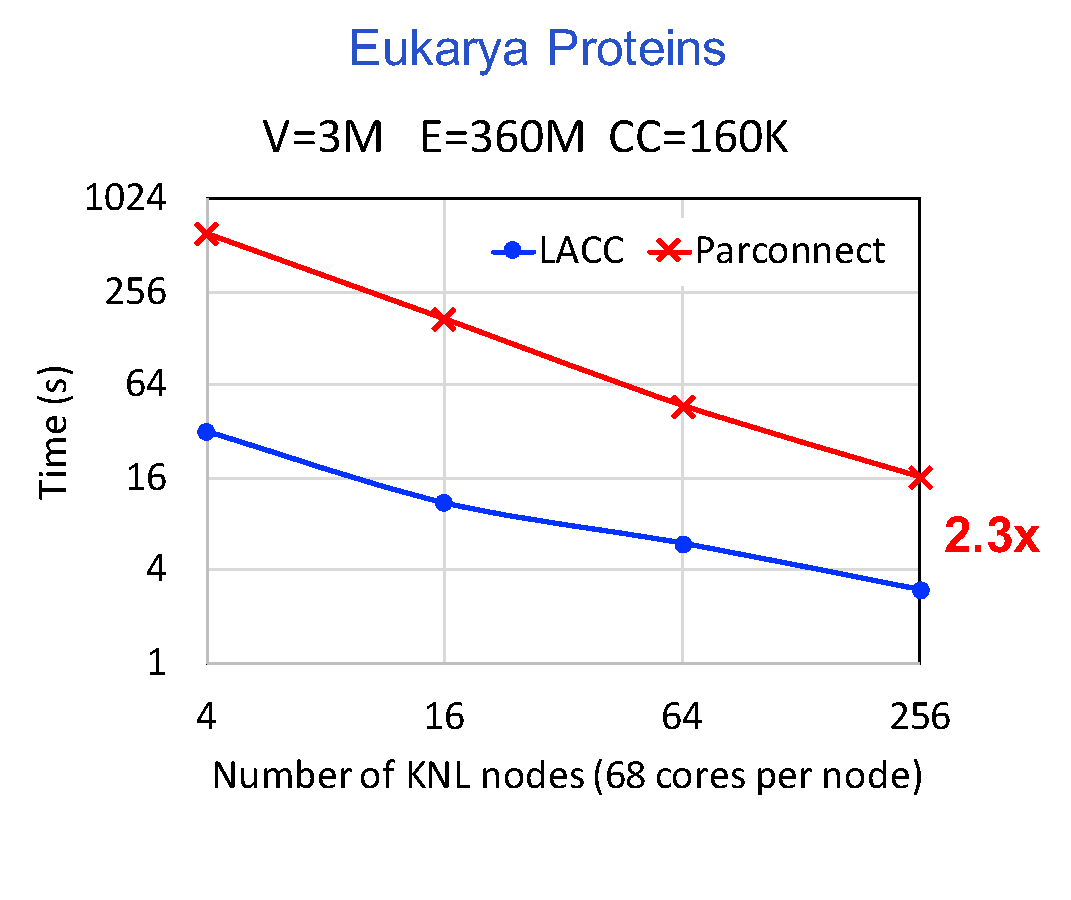
\includegraphics[scale=.5]{figures/eukarya} % requires the graphicx package
   \caption{Strong scaling of LACC and Parconnect when finding connected components in  the eukarya protein similarity network. }
   \label{fig:eukarya}
\end{figure}

\begin{figure}[!t]
   \centering
   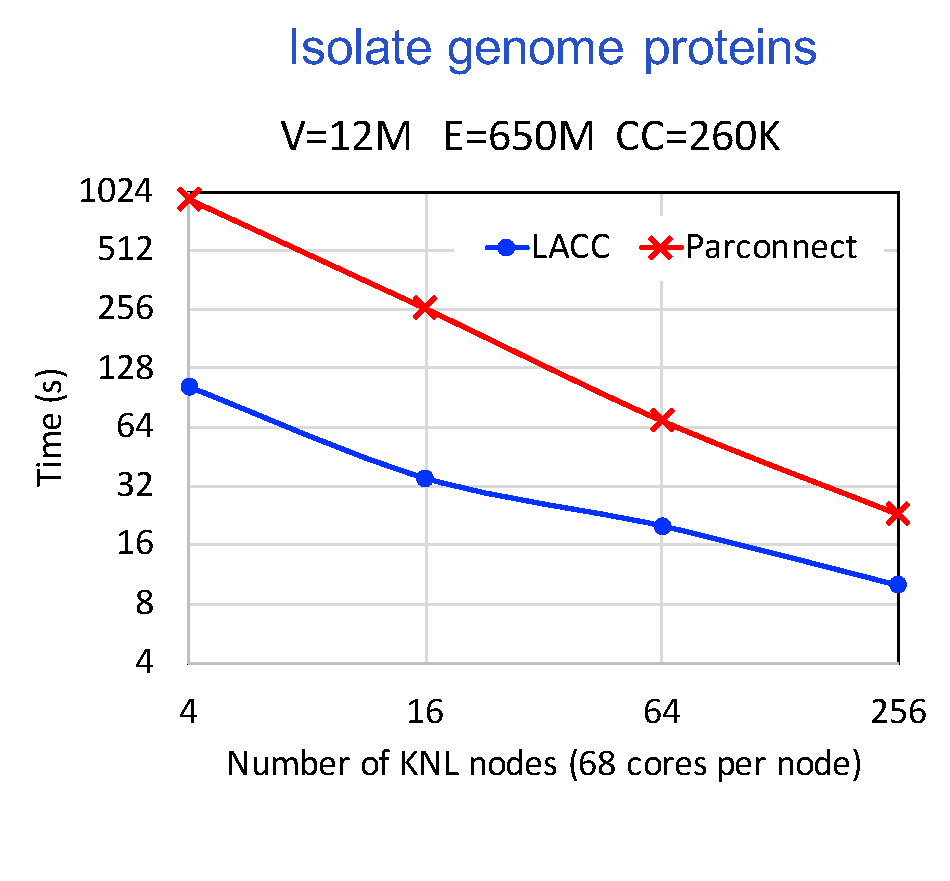
\includegraphics[scale=.5]{figures/isolates} % requires the graphicx package
   \caption{Strong scaling of LACC and Parconnect when finding connected components in  the isolate genomes protein similarity network. }
   \label{fig:isolates}
\end{figure}


\subsection{Performance of LACC with respect to the state-of-the-art}


\begin{figure*}[!t]
   \centering
   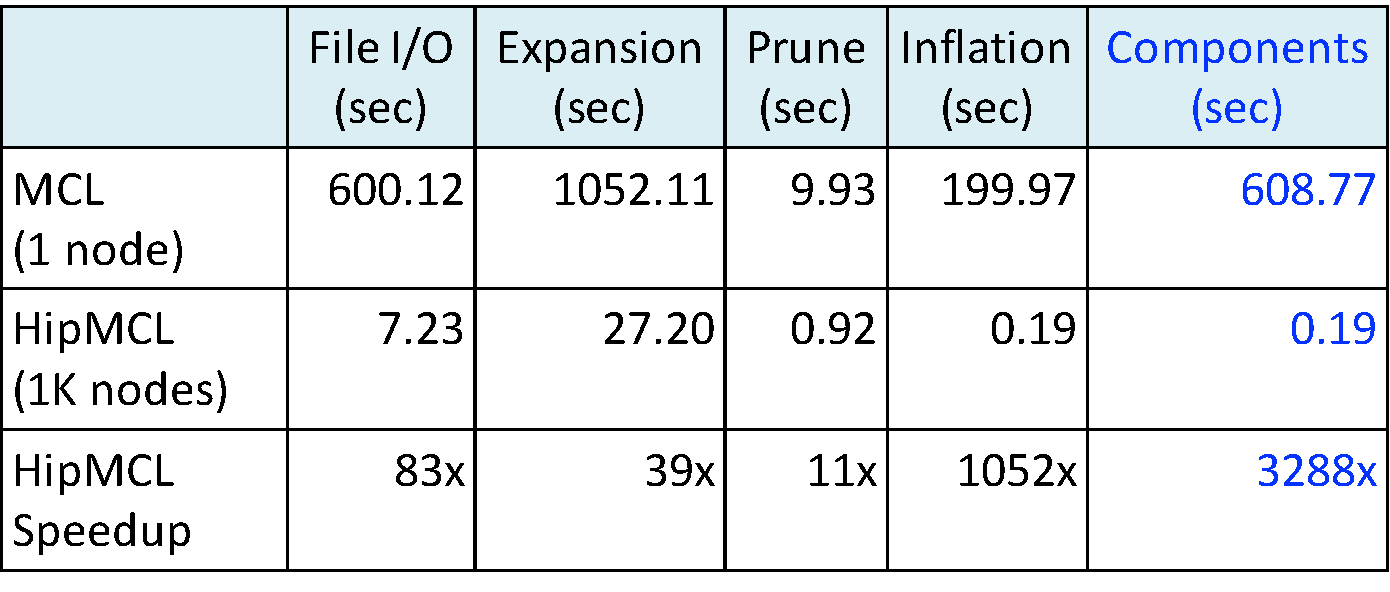
\includegraphics[scale=.5]{figures/hipmcl} % requires the graphicx package
   \caption{Performance improvement by LACC when used in HipMCL over the default shared-memory CC algorithm used in MCL. This result is obtained when clustering eukaryotic network with 3 million nodes and 359 million edges on NERSC/Edison.}
   \label{fig:hipmcl}
\end{figure*}

\subsection{Performance of LACC when used in Markov clustering}


